\section{User Roles}\label{sec:fa_roles}

\subsection{Variability Requirements}\label{sec:fa_roles_variability_requirements}

Authorization is one of the most sensitive areas of any closed software system: it ensures everyone does only what it should in order to guarantee everything works as expected. In a constantly evolving system, user roles have a strong tendency (\textbf{reference?}) to shift --- either because of new features or a new type of user is required in the system to perform specific tasks. In the context of \emph{escolinhas.pt} this problem ties itself with the ACL used: because of the diversity of roles (Fig.~\ref{fig:user_roles_current}) existent in the application and the three different usage plans, a lot of different rules are applied to determine if a user can or can not perform certain actions; allied to the growing number of features of the platform, this means that the authorization scheme has to be as flexible as possible to ensure minimal overhead when determining new types of permission sets.

\begin{figure}[H]
  \centering
  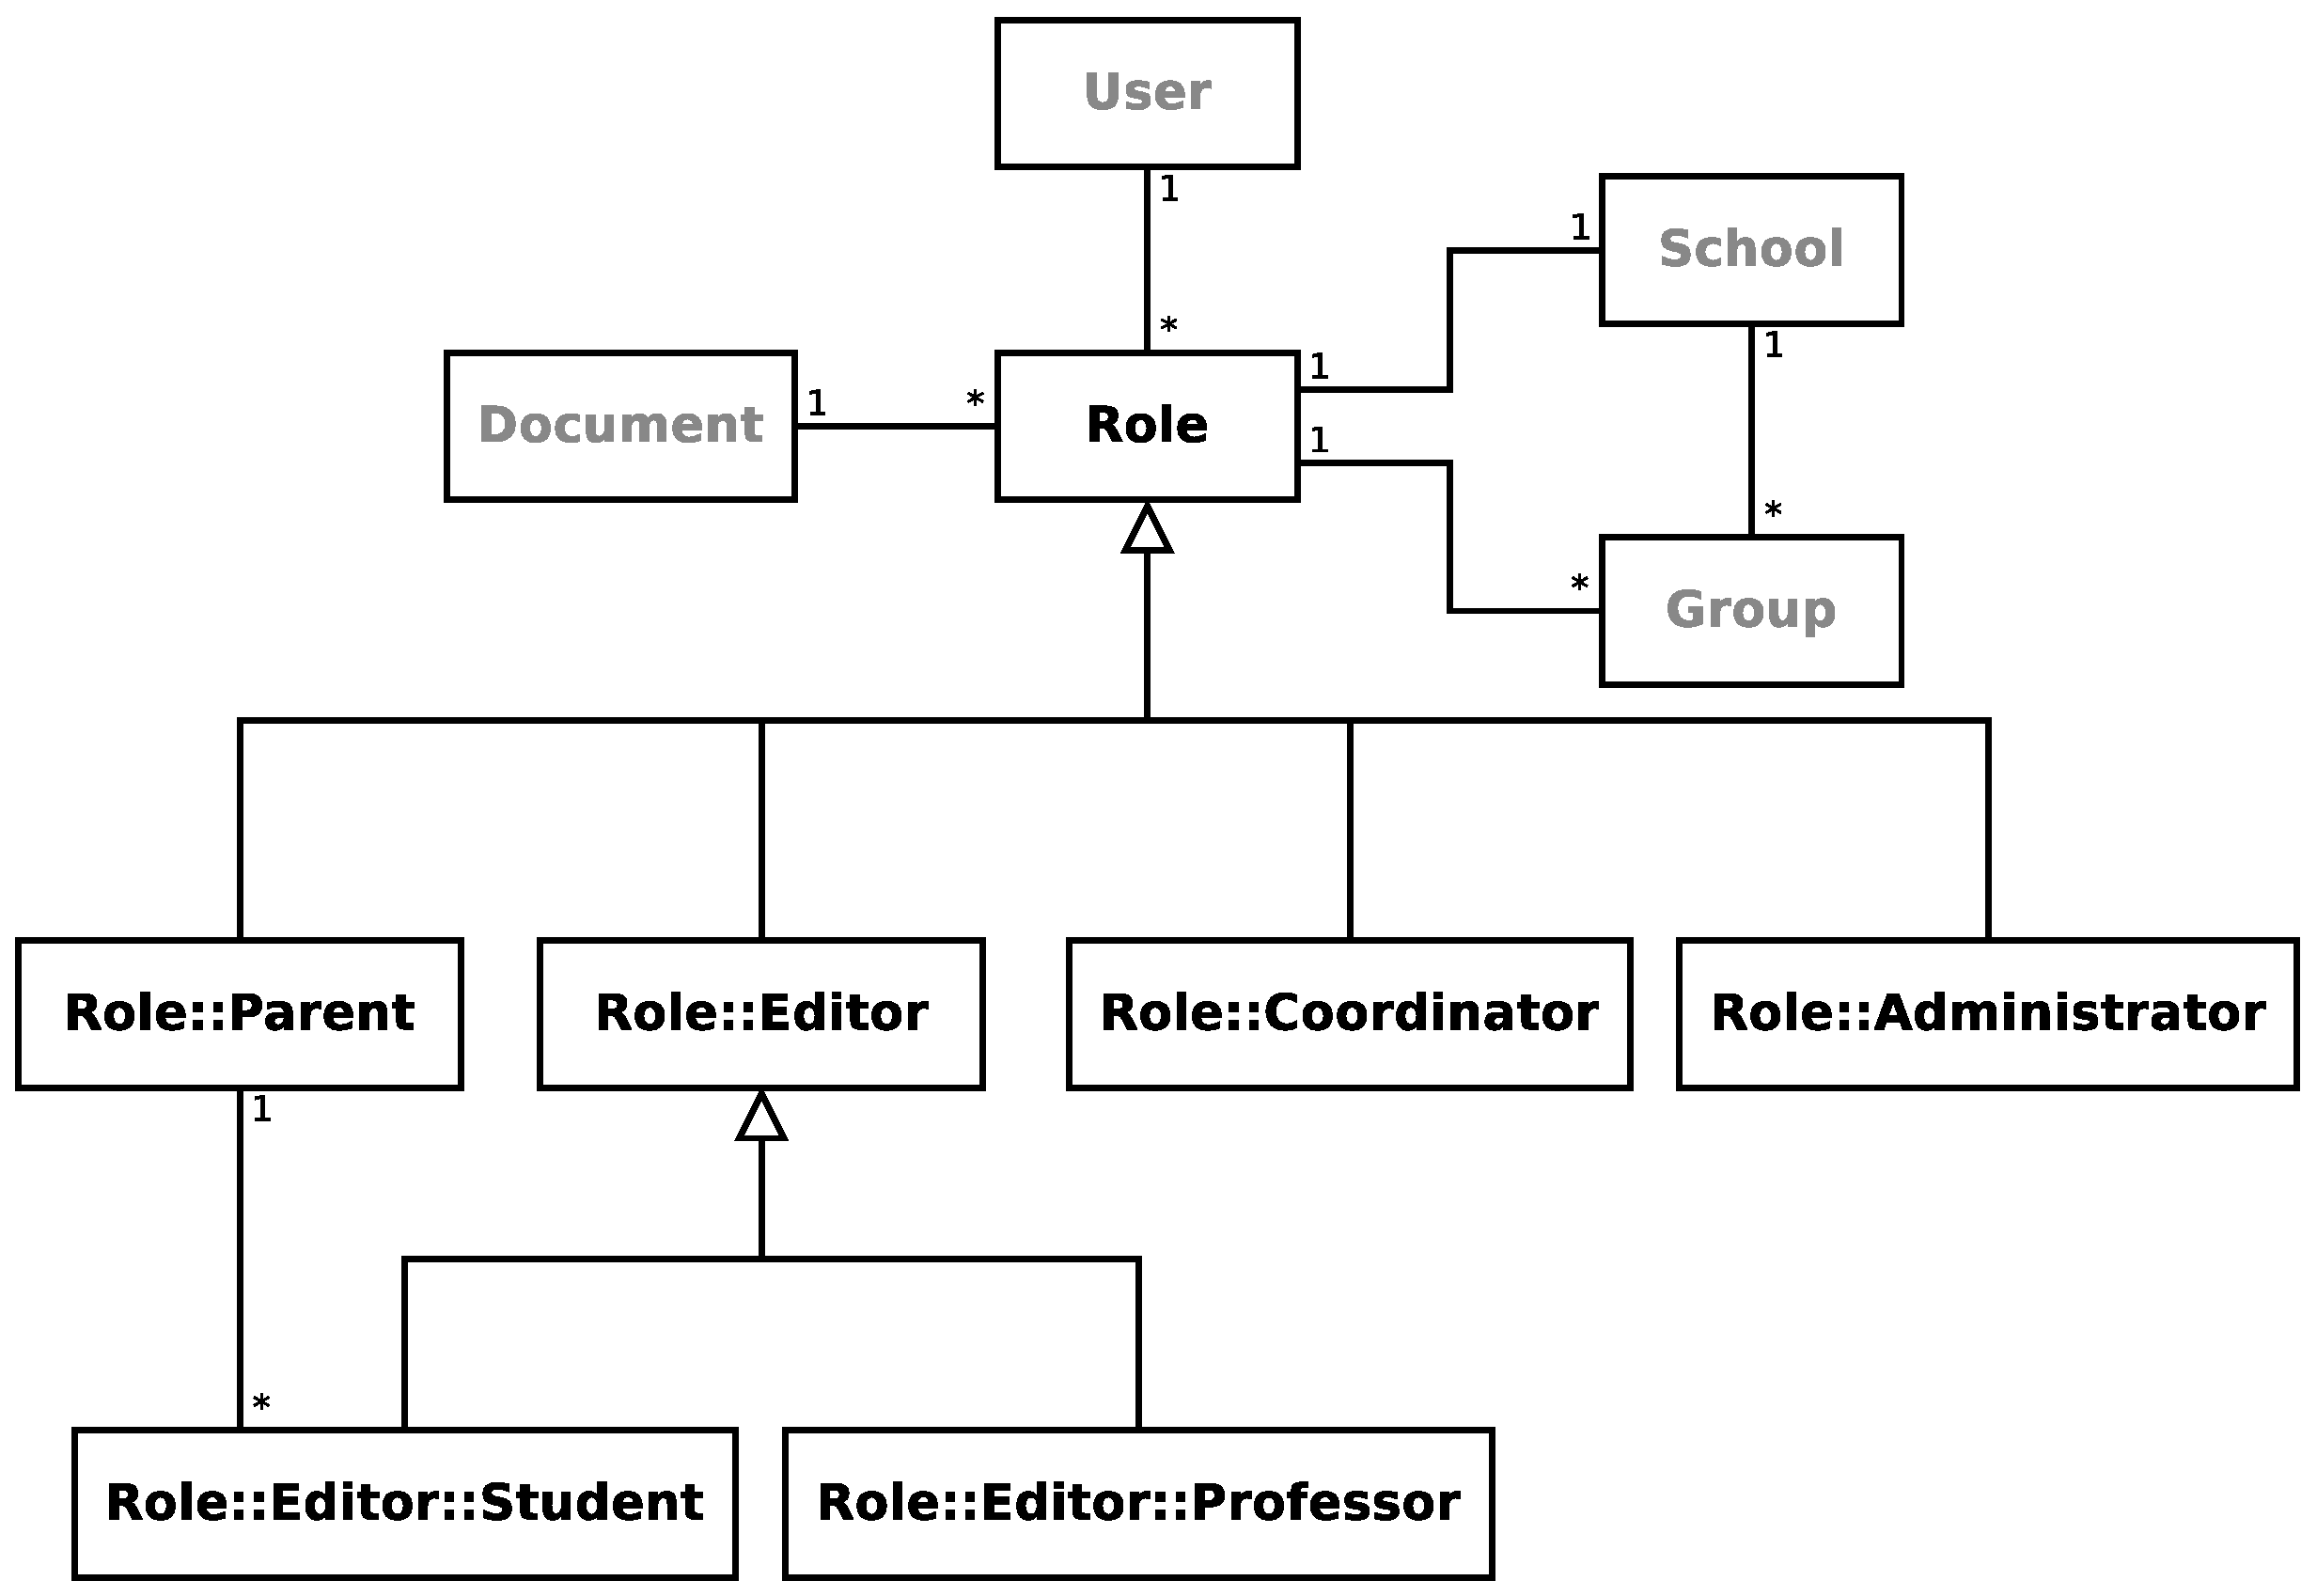
\includegraphics[width=130mm]{user_roles_current}
  \caption{Current User Roles Model}
  \label{fig:user_roles_current}
\end{figure}

\subsection{Candidate Patterns}\label{sec:fa_roles_candidate_patterns}

The current logic on roles and users states that a user may be a professor, a student, a parent, a coordinator (in which case it also has a professor role associated), or an administrator. Of these five different types of roles, only two of them are allowed editing privileges, which means that only students and professors have to ability to create and edit documents, which leads to an unnecessary level of complexity. If, for example, it was necessary to have a parent with editing privileges, a new Role, descendant of Role::Editor, would have to be created just for that user.

An obvious solution to this problem would be to tie a ``traditional'' \textsc{Access Control List} (as described in \cite{}) to the roles actually in use: this would allow to fine-tune each one of the users permissions and authorization sets while maintaining the codebase clean --- however, the logic surrounding authorization schemas and user roles is built around the \emph{CanCan} Ruby gem \cite{cancan}, which authorizes an user based on his or her roles, while keeping the necessary logic to a minimum. As such, the implementation of a full-fledged ACL could be considered as ``over-engineering'', as already perfectly capable authorization system is being used.

\subsection{Chosen Patterns \& Rationale}\label{sec:fa_roles_chosen_patterns_rationale}

As the implementation of an ACL was discarded in \ref{sec:fa_roles_candidate_patterns}, the best solution is to enhance the already present roles system: a flat Role hierarchy, as described in \cite{baumer_riehle_role_object} would allow for a more flexible authorization scheme, where a User could have one or more roles associated, depending on what actions he would be allowed to do, as shown on Fig.~\ref{fig:user_roles_conceptual}. This also makes the task of creating new roles with different authorization schemes much easier, as there is not a need to conform to any special hierarchy scheme: a new role simply means a new type of user. This clearly constrasts with the previous role's logic, where a multi-level hierarchy was in place.

\begin{figure}[H]
  \centering
  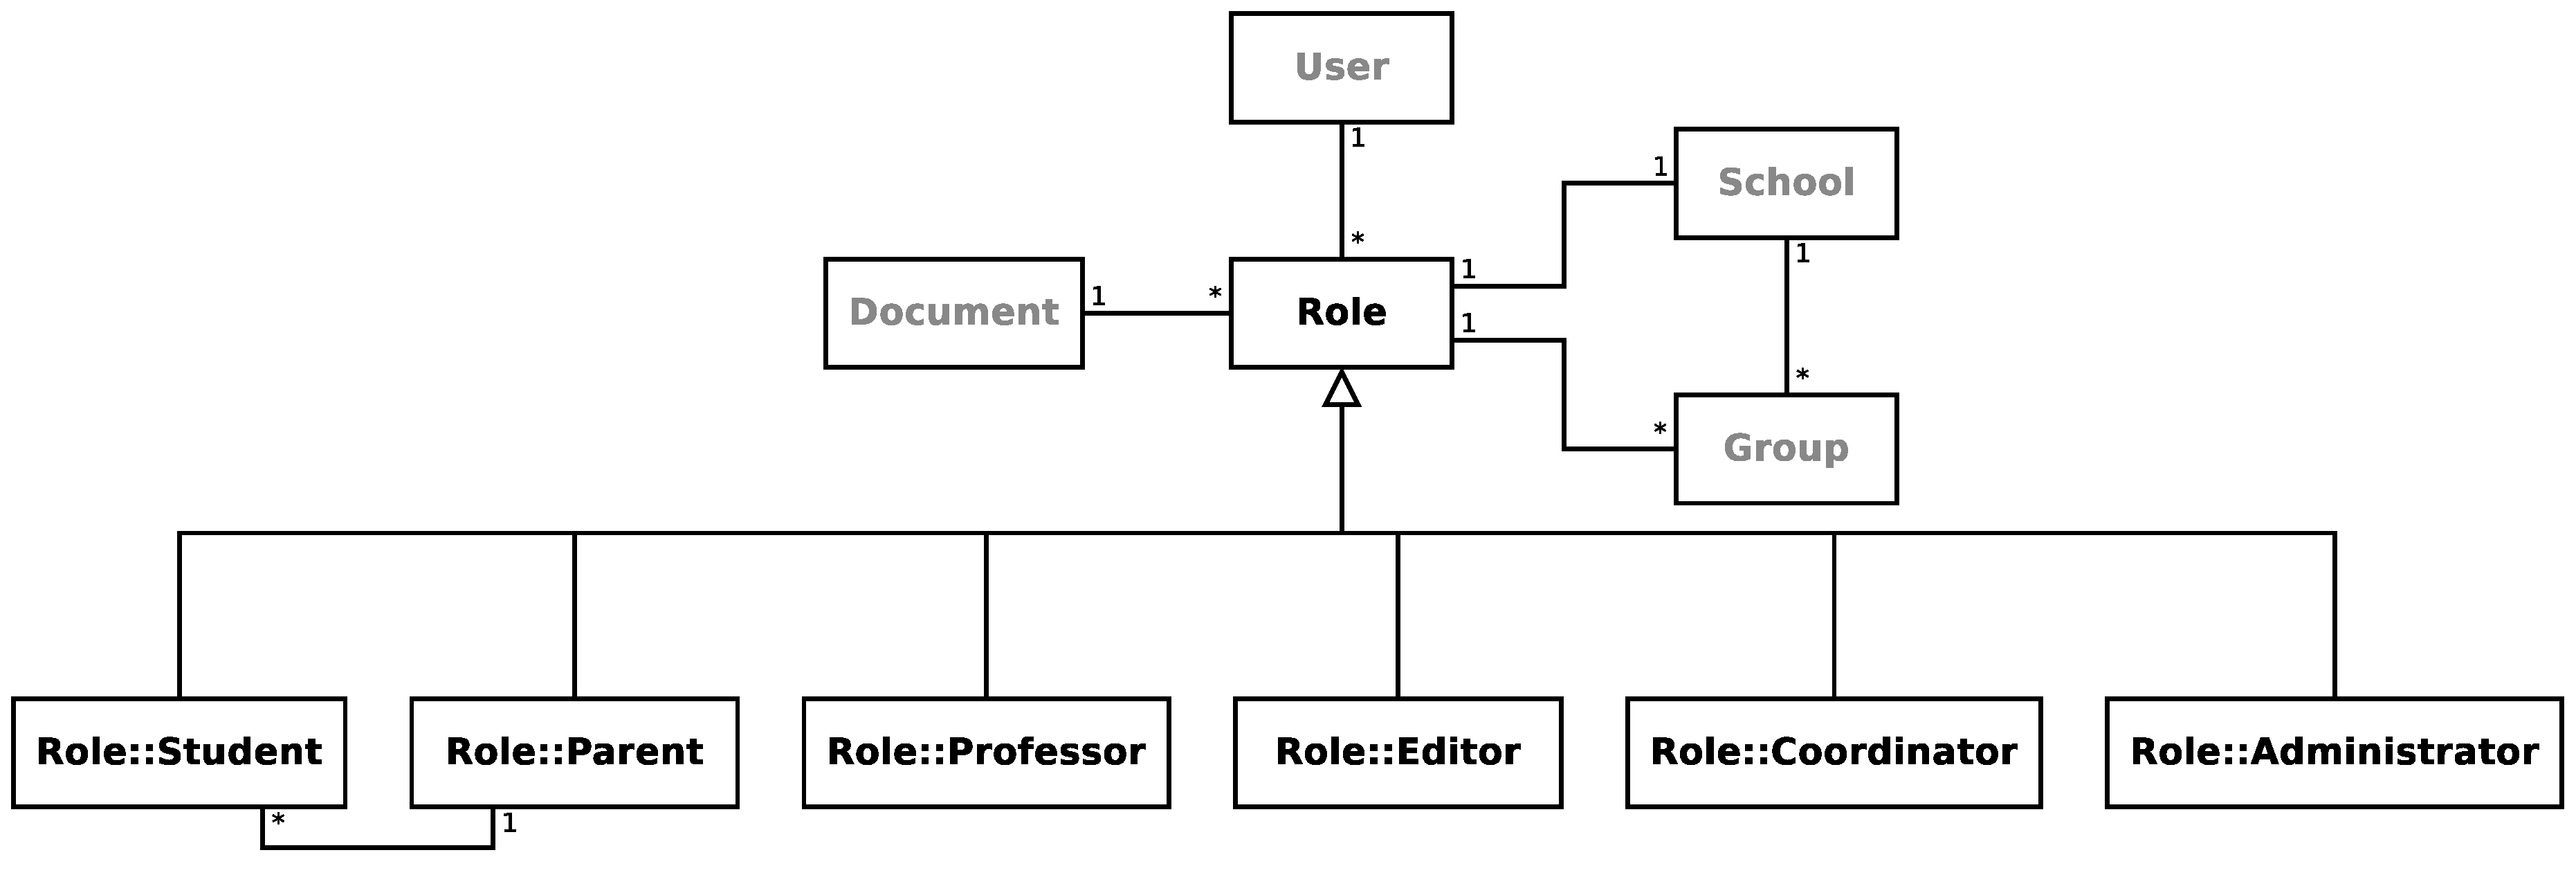
\includegraphics[width=160mm]{user_roles_conceptual}
  \caption{Conceptual User Roles Model}
  \label{fig:user_roles_conceptual}
\end{figure}

\subsection{Implementation}\label{sec:fa_roles_implementation}

The refactoring of the roles infrastructure was of very low impact, as codebase and database schema are regarded. The hierarchy of Role classes was flattened, keeping it at only two levels: a generic, non-instantiable class \emph{Role}, and all of its currently existent subclasses: \emph{Editor, Parent, Student, Professor, Coordinator} and \emph{Administrator}. Then, the existent rules were adapted to fit this new hierarchy. The last pertains to migrating the current data to the new role organization --- it entails analysing each user current roles and performing the adequate substitutions from the previous roles schema. 

\subsection{Impact Analysis}\label{sec:fa_roles_impact_analysis}
